\documentclass[a4paper,7pt]{jsarticle}
\usepackage{stdrep}
\usepackage{url}

\author{青木大祐}
\title{ソフトウェアサイエンスセミナ資料 \\ Voynich Manuscript}

\usepackage{fancybox}	% required for `\ovalbox' (yatex added)
\usepackage{ascmac}	% required for `\screen' (yatex added)
\usepackage{graphicx}	% required for `\includegraphics' (yatex added)
\begin{document}
\maketitle
\section{概要}

ヴォイニッチ手稿(Voynich Manuscript)についての概要を
\url{http://voynich.com/}より引用する。
\begin{screen}
 この書物は「The Most Mysterious Manuscript in the World」とも呼ばれている、世界で最もミステリアスな書物である。表紙やいくつかのページは紛失しているが、およそ230ページからなる古文書である。見たこともない不思議なアルファベットで書かれていて、さらに不思議な植物の絵も描かれている。ヴォイニッチ手稿とは発見者Wilfrid M. Voynichにちなんで名付けられた。彼は1912年イタリアのモンドラゴーネ寺院でそれを発見したといわれている。 その作者、年代、たどってきた歴史ははっきりしていないが、14~16世紀に作られたと考えられている。間接的な証拠からおそらくジョン・ディーやルドルフ2世も一時所有していたであろう。Wilfrid M. Voynich死後、古書商ハンス・クラウスの手に渡り、彼は1960年に16万ドルで売り出すも買い手はつかず、1969年イェール大学ベイニック図書館に寄贈された。 
\end{screen}
ヴォイニッチ手稿に書かれている文章は、未だに何の言語で書かれているのか解
明されておらず、また当然内容についても同様である。これに関して、幾つかの
仮説が唱えられている。
\begin{itemize}
 \item 完全に未知の言語で書かれている説
       \begin{itemize}
        \item 今では失われた言語
        \item 特殊な用途に用いられた言語
        \item 宇宙人が残した文書(!)
       \end{itemize}
 \item 暗号で書かれている説
 \item 言語も内容もデタラメの偽書である説
       \begin{itemize}
        \item 当時の人間が、貴重なものとして高値で売るために制作した
        \item この手稿を発見したというVoinichによって制作された
       \end{itemize}
\end{itemize}
また、この書物が何を記述しているのかについても議論が行われており、代表的
なものとして次のような説がある。
\begin{itemize}
 \item 錬金術や魔術などの手法をまとめている
 \item 薬草などの植物に関する図鑑
 \item 単なる偽書なので内容は無い
\end{itemize}
この謎めいた書物について、どのようにして研究が行われてきたのかを軽く紹介
する。

\section{今までに行われてきた研究}
\subsection{科学的なアプローチ}
ヴォイニッチ手稿の紙やインクを科学的に分析することで、作られた年代を特定
しようという試み。アリゾナ大学で行われた炭素分析によって、羊皮紙が作られ
た年代は1404年から1438年であると特定されている。
\subsection{歴史学的なアプローチ}
昔の書簡などの資料から、1600年代にはヴォイニッチ手稿の存在が確認されている。つまり、1900年台にVoynichによって作成された偽書という説は否定された。
\subsection{語彙統計学的なアプローチ}
言語学的な検知から、他の言語と同じような性質を見出すことが出来るかという
研究である。単語や文字の出現頻度・エントロピーなどから、この文章は自然言
語に近い性質を示し、暗号ではないようだという結論が出ている。
また、この手稿が制作されたと考えられている1400年代には言語学は発達してお
らず、単語の出現頻度の傾向などは研究されていなかった。それにもかかわらず、一般的な自然言語と同様の傾向が見られることから、これは人為的に作られたデタラメではないであろうと考えられる。

\subsection{情報科学的なテキスト処理によるアプローチ}
これまでの既存研究に加え、現代では計算機を解析に用いた研究が始まっている。
今までは手作業で行われてきた統計も簡単に行えるようになり、また自然言語処
理の手法を取り入れることで、新たな突破口が開けるのではないかという期待が
持たれている。\\

既に成果を上げている研究として「文書クラスタリングによる未解読文書の解
読可能性の判定 - ヴォイニッチ写本の事例」という論文があり、「本文の構造
と挿絵・ページから推測される構造が一致することが明らかになった。つまり、
ヴォイニッチ写本は一貫性のある構造を持つ文書であり、捏造文書ではない可能
性が高いと判断できる」という結論を出している。

\newpage
\section{おまけ}
f78r
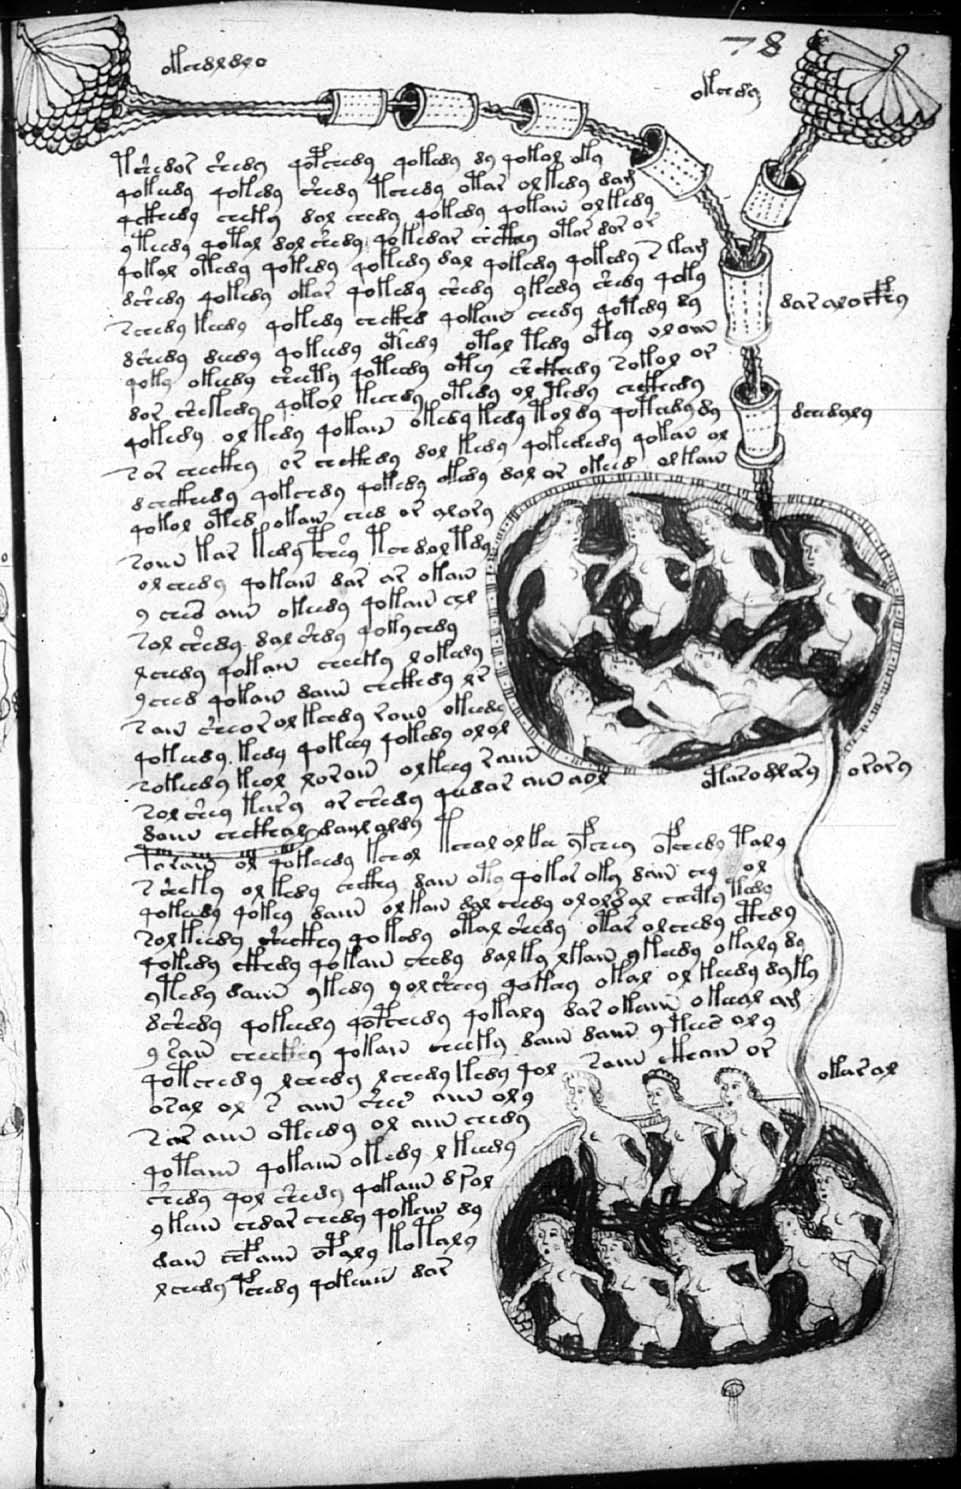
\includegraphics[width=15cm]{f78r.jpg}
\newpage
f89r1
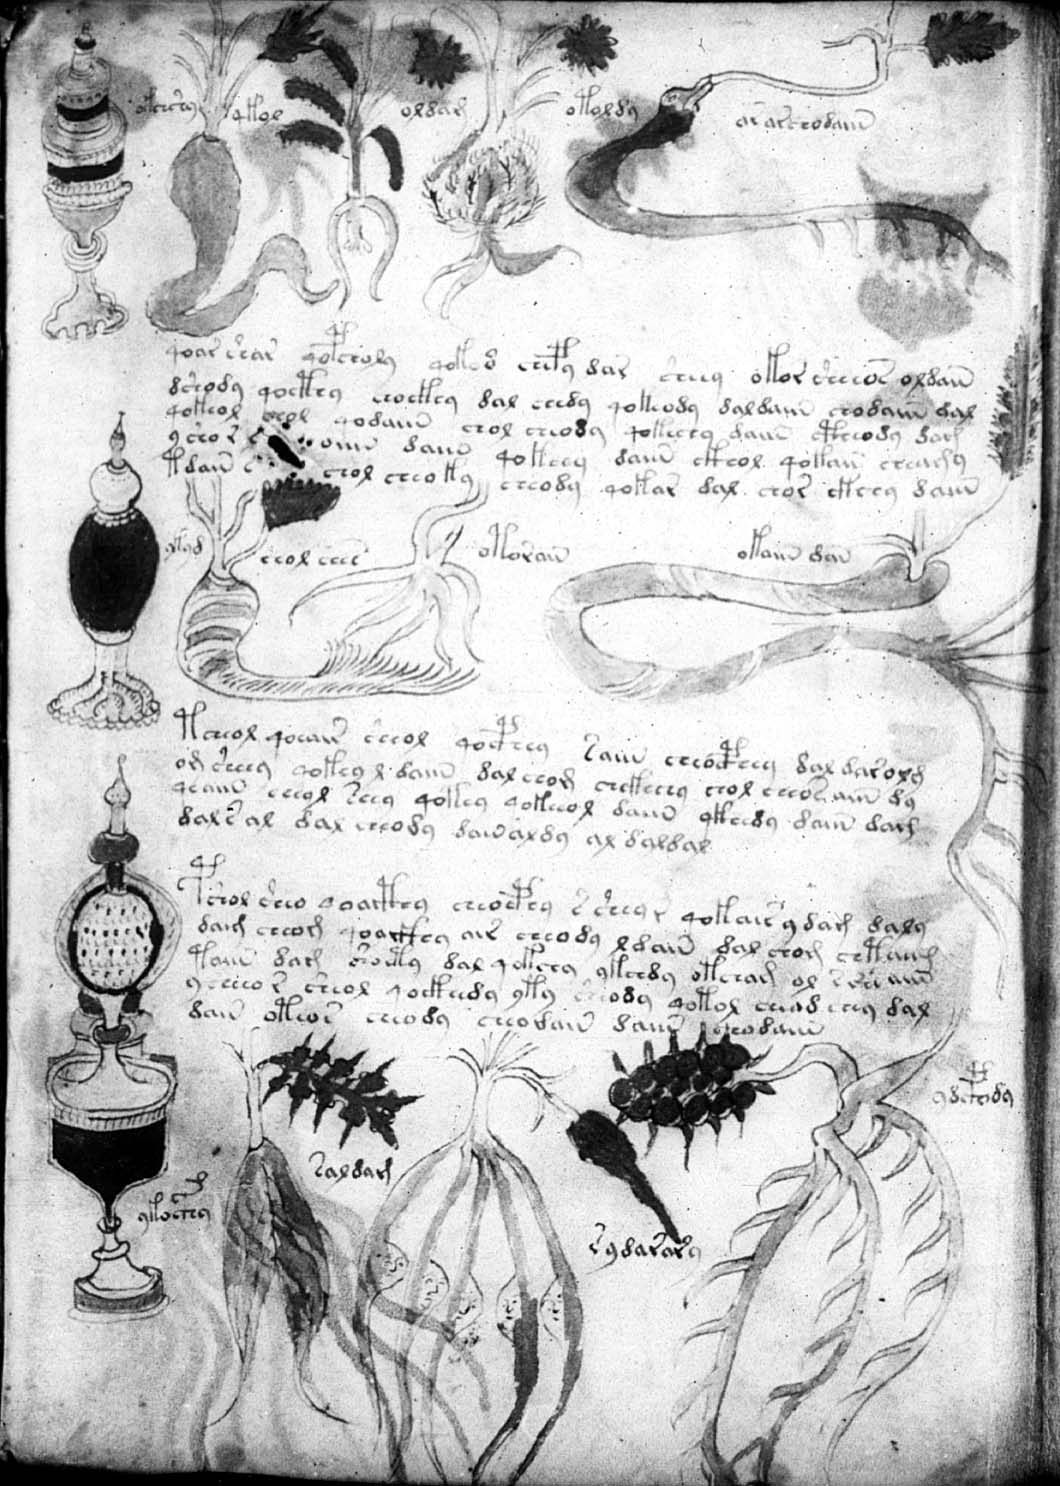
\includegraphics[width=15cm]{f89r1.jpg}

\end{document}